\documentclass[12pt,letterpaper]{article}
\usepackage{graphicx,textcomp}
\usepackage{natbib}
\usepackage{setspace}
\usepackage{fullpage}
\usepackage{color}
\usepackage[reqno]{amsmath}
\usepackage{amsthm}
\usepackage{fancyvrb}
\usepackage{amssymb,enumerate}
\usepackage[all]{xy}
\usepackage{endnotes}
\usepackage{lscape}
\newtheorem{com}{Comment}
\usepackage{float}
\usepackage{hyperref}
\newtheorem{lem} {Lemma}
\newtheorem{prop}{Proposition}
\newtheorem{thm}{Theorem}
\newtheorem{defn}{Definition}
\newtheorem{cor}{Corollary}
\newtheorem{obs}{Observation}
\usepackage[compact]{titlesec}
\usepackage{dcolumn}
\usepackage{tikz}
\usetikzlibrary{arrows}
\usepackage{multirow}
\usepackage{xcolor}
\newcolumntype{.}{D{.}{.}{-1}}
\newcolumntype{d}[1]{D{.}{.}{#1}}
\definecolor{light-gray}{gray}{0.65}
\usepackage{url}
\usepackage{listings}
\usepackage{color}
\usepackage{caption}

\definecolor{codegreen}{rgb}{0,0.6,0}
\definecolor{codegray}{rgb}{0.5,0.5,0.5}
\definecolor{codepurple}{rgb}{0.58,0,0.82}
\definecolor{backcolour}{rgb}{0.95,0.95,0.92}

\lstdefinestyle{mystyle}{
	backgroundcolor=\color{backcolour},   
	commentstyle=\color{codegreen},
	keywordstyle=\color{magenta},
	numberstyle=\tiny\color{codegray},
	stringstyle=\color{codepurple},
	basicstyle=\footnotesize,
	breakatwhitespace=false,         
	breaklines=true,                 
	captionpos=b,                    
	keepspaces=true,                 
	numbers=left,                    
	numbersep=5pt,                  
	showspaces=false,                
	showstringspaces=false,
	showtabs=false,                  
	tabsize=2
}
\lstset{style=mystyle}
\newcommand{\Sref}[1]{Section~\ref{#1}}
\newtheorem{hyp}{Hypothesis}

\title{Replication Project: Oil, Islam, and Women}
\date{April 1, 2026}
\author{Kate Cox}


\begin{document}
	\maketitle
	\section*{Original Study}
	\vspace{.25cm}
	
	\subsection*{Theory}
	
	\vspace{.25cm}
	
	\noindent The study Oil, Islam, and Women by Michael L. Ross proposes that women in the Middle East have been held back from the workforce not by Islamic traditions, as has been the primary theory in the literature, but by oil. This questions another idea documented in existing literature, that economic growth benefits gender equality.
	
	\vspace{.5cm}
	
	\noindent The study proposes that different types of economic growth have different impacts on gender equality in the labor force. He proposes that oil and mineral extraction leaves few opportunities for women, leading to impacts on their labor and, therefore, social and political inclusion. He believes that, in contrast to the negative effect of an oil-based economy on women, export-oriented industries, specifically textiles, are positive for women's economic growth. He suggests that, if these findings hold, they may have implications for the way that the U.S. considers oil transactions. 
	
	\vspace{.5cm}
	 
	\subsection*{Method}

	\vspace{.25cm}
	
	\noindent Ross analyzed oil production and female employment data from 1960 until 2002. He looked at first-differences models with fixed effects to examines variations over time in the same state. He also looked at cross-national models to examine variations between states. His tables include both GLS and OLS regressions.
	
	\subsection*{Variables}
	
	\vspace{.25cm}
	
	\noindent The outcome variable is \textit{Oil Rents Per Capita}. The  predictor variables are \textit{Female Labor Force Participation} and female political influence measured by \textit{Female Seats} (the percentage of seats held by women in the country's parliament) and \textit{Female Ministers} (the percentage of the ministerial positions held by women). This study uses 2002 data. The study controls for other variables including \textit{Income}, \textit{Income Squared}, \textit{Middle East} (whether the country is in the Middle East), \textit{Islam} (the proportion of the country that is Muslim),\textit{Communist} (a dummy variable indicating whether or not the country is Communist), \textit{Working Age} (the proportion of the population between 15 and 64), \textit{Proportional Representation} (a dummy variable for states with proportional representation in parliament), \textit{Closed List}, (a dummy variable for electoral systems with closed lists), and \textit{Polity} (a scale to measure democracy level).

	\subsection*{Data}
	
	\vspace{.25cm}
	
	\noindent There are 2 data sources provided for replication, data\_long and data\_short.

	\lstinputlisting[language=R, firstline=11, lastline=12]{replication_KC.R}
	
	\subsection*{Table 1}
	\lstinputlisting[language=R, firstline=16, lastline=61]{replication_KC.R}
	
\begin{table}[!htbp] \centering 
	\caption*{Table 1. Pooled Time-Series Cross-national Regressions, with First Differences and Fixed Effects} 
	\label{} 
	\begin{tabular}{@{\extracolsep{5pt}}lcccc} 
		\\[-1.8ex]\hline 
		\hline \\[-1.8ex] 
		& \multicolumn{4}{c}{\textit{Dependent variable:}} \\ 
		\cline{2-5} 
		\\[-1.8ex] & \multicolumn{4}{c}{Female Labor Force Participation, 1960-2002} \\ 
		\\[-1.8ex] & \multicolumn{3}{c}{\textit{generalized}} & \textit{OLS} \\ 
		& \multicolumn{3}{c}{\textit{least squares}} & \textit{} \\ 
		\\[-1.8ex] & (1) & (2) & (3) & (4)\\ 
		\hline \\[-1.8ex] 
		Income (log) & $-$0.014 & $-$0.042 & $-$0.013 & $-$0.051 \\ 
		& (0.033) & (0.034) & (0.028) & (0.047) \\ 
		& & & & \\ 
		Income squared (log) & 0.018 & 0.051 & 0.018 & 0.021 \\ 
		& (0.033) & (0.034) & (0.029) & (0.048) \\ 
		& & & & \\ 
		Working Age & 0.107$^{***}$ & 0.106$^{***}$ & 0.067$^{***}$ & 0.177$^{***}$ \\ 
		& (0.022) & (0.022) & (0.021) & (0.013) \\ 
		& & & & \\ 
		Oil Rents per capita &  & $-$0.028$^{***}$ & $-$0.017$^{*}$ & $-$0.049$^{***}$ \\ 
		&  & (0.007) & (0.010) & (0.011) \\ 
		& & & & \\ 
		Constant & $-$0.498 & $-$0.497 & $-$0.536 & $-$0.404$^{**}$ \\ 
		& (0.364) & (0.364) & (0.400) & (0.179) \\ 
		& & & & \\ 
		\hline \\[-1.8ex] 
		Observations & 5,234 & 5,234 & 5,168 & 5,395 \\ 
		R$^{2}$ &  &  &  & 0.562 \\ 
		Adjusted R$^{2}$ &  &  &  & 0.544 \\ 
		Log Likelihood & $-$3,536.648 & $-$3,528.950 & $-$2,474.278 &  \\ 
		Akaike Inf. Crit. & 7,405.295 & 7,391.900 & 5,278.555 &  \\ 
		Bayesian Inf. Crit. & 8,494.742 & 8,487.910 & 6,359.345 &  \\ 
		\hline 
		\hline \\[-1.8ex] 
		\textit{Note:}  & \multicolumn{4}{r}{$^{*}$p$<$0.1; $^{**}$p$<$0.05; $^{***}$p$<$0.01} \\ 
	\end{tabular} 
\end{table} 

	\subsection*{Table 2}

	\lstinputlisting[language=R, firstline=65, lastline=88]{replication_KC.R}

\begin{table}[!htbp] \centering 
	\caption*{Table 2. Cross-national Regressions on Female Labor Force} 
	\label{} 
	\small 
	\begin{tabular}{@{\extracolsep{1pt}}lcccc} 
		\\[-1.8ex]\hline 
		\hline \\[-1.8ex] 
		& \multicolumn{4}{c}{\textit{Dependent variable:}} \\ 
		\cline{2-5} 
		\\[-1.8ex] & \multicolumn{4}{c}{Female Nonagricultural Labor Force Participation, 1993-2002} \\ 
		\\[-1.8ex] & (1) & (2) & (3) & (4)\\ 
		\hline \\[-1.8ex] 
		Income (log) & $-$1.334 & $-$1.499$^{*}$ & $-$1.757$^{**}$ & $-$1.864$^{**}$ \\ 
		& (0.843) & (0.874) & (0.852) & (0.878) \\ 
		& & & & \\ 
		Income squared (log) & 1.615$^{**}$ & 1.735$^{**}$ & 2.053$^{**}$ & 2.122$^{**}$ \\ 
		& (0.798) & (0.823) & (0.805) & (0.824) \\ 
		& & & & \\ 
		Working Age & $-$0.386$^{***}$ & $-$0.395$^{***}$ & $-$0.340$^{**}$ & $-$0.350$^{**}$ \\ 
		& (0.141) & (0.143) & (0.139) & (0.142) \\ 
		& & & & \\ 
		Middle East & $-$0.521$^{***}$ & $-$0.407$^{***}$ & $-$0.413$^{***}$ & $-$0.326$^{***}$ \\ 
		& (0.083) & (0.117) & (0.084) & (0.117) \\ 
		& & & & \\ 
		Communist & 0.290$^{***}$ & 0.292$^{***}$ & 0.284$^{***}$ & 0.286$^{***}$ \\ 
		& (0.104) & (0.104) & (0.103) & (0.104) \\ 
		& & & & \\ 
		Islam &  & $-$0.170 &  & $-$0.139 \\ 
		&  & (0.113) &  & (0.116) \\ 
		& & & & \\ 
		Oil Rents per capita &  &  & $-$0.225$^{***}$ & $-$0.210$^{***}$ \\ 
		&  &  & (0.053) & (0.055) \\ 
		& & & & \\ 
		Constant & $-$0.012 & $-$0.014 & $-$0.010 & $-$0.012 \\ 
		& (0.062) & (0.062) & (0.060) & (0.060) \\ 
		& & & & \\ 
		\hline \\[-1.8ex] 
		Observations & 167 & 167 & 167 & 167 \\ 
		R$^{2}$ & 0.382 & 0.396 & 0.417 & 0.427 \\ 
		Adjusted R$^{2}$ & 0.363 & 0.374 & 0.395 & 0.401 \\ 
		Residual Std. Error & 0.800 & 0.793 & 0.780 & 0.776 \\ 
		F Statistic & 19.889$^{***}$ & 17.501$^{***}$ & 19.086$^{***}$ & 16.898$^{***}$ \\ 
		\hline 
		\hline \\[-1.8ex] 
		\textit{Note:}  & \multicolumn{4}{r}{$^{*}$p$<$0.1; $^{**}$p$<$0.05; $^{***}$p$<$0.01} \\ 
	\end{tabular} 
\end{table} 

\newpage

\subsection*{Table 3}
\lstinputlisting[language=R, firstline=93, lastline=116]{replication_KC.R}

Note: Attempting to replicate Table 3 (which was not included in the Anderson and Hill replication code) revealed problems with Ross's provided replication data and lack of transparency. For many variables, he only provided the Z-scores, not the raw numbers. This made it impossible to replicate his original method as he did not clarify which countries he put in each category. This code strikes a balance between constraining itself so that it is performing similarly to Ross's (making similar choices about what countries to drop and which countries belong in each category), while still performing actual calculations using the data available.

\vspace{.25cm}

\begin{verbatim}
	[1] "TABLE 3. Parliamentary Seats Held by Woman, 2002 (percentage)"
	Group Oil_Rich Oil_Poor
	1           High Income     15.7     17.9
	2            Low Income     11.6     13.0
	3           Middle East      5.5      6.5
	4 Non-Middle East (all)     17.8     15.7
	5 Non-Middle East (dev)     13.9     14.5
	6               Islamic      7.2      9.8
	7     Non-Islamic (all)     19.3     16.5
	8     Non-Islamic (dev)     15.0     15.2
\end{verbatim}

\subsection*{Table 4}

\lstinputlisting[language=R, firstline=120, lastline=148]{replication_KC.R}

\begin{table*}[!htbp] \centering 
	\caption*{Table 4. Cross-national Regressions on Female Seats in Parliament} 
	\label{} 
	\small 
	\begin{tabular}{@{\extracolsep{-15pt}}lcccccccc} 
		\\[-1.8ex]\hline 
		\hline \\[-1.8ex] 
		& \multicolumn{8}{c}{\textit{Dependent variable:}} \\ 
		\cline{2-9} 
		\\[-1.8ex] & \multicolumn{8}{c}{Parliamentary Seats Held by Women (percent), 2002} \\ 
		\\[-1.8ex] & (1) & (2) & (3) & (4) & (5) & (6) & (7) & (8)\\ 
		\hline \\[-1.8ex] 
		Income (log) & 0.311$^{***}$ & 0.259$^{***}$ & 0.365$^{***}$ & 0.320$^{***}$ & 0.390$^{***}$ & 0.367$^{***}$ & 0.779$^{***}$ & 0.329$^{***}$ \\ 
		& (0.082) & (0.092) & (0.083) & (0.094) & (0.094) & (0.089) & (0.137) & (0.088) \\ 
		& & & & & & & & \\ 
		Middle East & $-$0.378$^{***}$ & $-$0.261$^{***}$ & $-$0.278$^{***}$ & $-$0.193$^{**}$ & $-$0.233$^{***}$ & $-$0.253$^{***}$ & $-$0.182 & $-$0.080 \\ 
		& (0.062) & (0.084) & (0.060) & (0.080) & (0.083) & (0.077) & (0.143) & (0.095) \\ 
		& & & & & & & & \\ 
		Islam &  & $-$0.178$^{*}$ &  & $-$0.139 & $-$0.180$^{*}$ & $-$0.144 & $-$0.123 & $-$0.103 \\ 
		&  & (0.092) &  & (0.089) & (0.097) & (0.096) & (0.175) & (0.087) \\ 
		& & & & & & & & \\ 
		Oil Rents per Capita &  &  & $-$0.233$^{***}$ & $-$0.218$^{***}$ & $-$0.258$^{***}$ & $-$0.238$^{***}$ & $-$0.317$^{***}$ & $-$0.152$^{**}$ \\ 
		&  &  & (0.070) & (0.066) & (0.076) & (0.069) & (0.087) & (0.070) \\ 
		& & & & & & & & \\ 
		Polity &  &  &  &  & $-$0.158 & $-$0.298$^{***}$ & $-$0.294$^{**}$ &  \\ 
		&  &  &  &  & (0.103) & (0.101) & (0.149) &  \\ 
		& & & & & & & & \\ 
		Proportional Representation &  &  &  &  &  & 0.316$^{***}$ & 0.013 &  \\ 
		&  &  &  &  &  & (0.073) & (0.133) &  \\ 
		& & & & & & & & \\ 
		Closed List &  &  &  &  &  &  & 0.268$^{***}$ &  \\ 
		&  &  &  &  &  &  & (0.091) &  \\ 
		& & & & & & & & \\ 
		Female Labor Force Participation &  &  &  &  &  &  &  & 0.309$^{***}$ \\ 
		&  &  &  &  &  &  &  & (0.084) \\ 
		& & & & & & & & \\ 
		Constant & $-$0.013 & $-$0.018 & $-$0.015 & $-$0.018 & $-$0.016 & $-$0.022 & 0.034 & $-$0.015 \\ 
		& (0.070) & (0.069) & (0.068) & (0.068) & (0.068) & (0.064) & (0.105) & (0.066) \\ 
		& & & & & & & & \\ 
		\hline \\[-1.8ex] 
		Observations & 161 & 161 & 161 & 161 & 161 & 161 & 88 & 160 \\ 
		R$^{2}$ & 0.212 & 0.227 & 0.255 & 0.264 & 0.275 & 0.346 & 0.403 & 0.328 \\ 
		Adjusted R$^{2}$ & 0.202 & 0.212 & 0.240 & 0.245 & 0.252 & 0.320 & 0.350 & 0.306 \\ 
		Residual Std. Error & 0.893 & 0.888 & 0.872 & 0.869 & 0.865 & 0.824 & 0.828 & 0.835 \\ 
		F Statistic & 21.271$^{***}$ & 15.374$^{***}$ & 17.885$^{***}$ & 13.966$^{***}$ & 11.754$^{***}$ & 13.562$^{***}$ & 7.702$^{***}$ & 15.027$^{***}$ \\ 
		\hline 
		\hline \\[-1.8ex] 
		\textit{Note:}  & \multicolumn{8}{r}{$^{*}$p$<$0.1; $^{**}$p$<$0.05; $^{***}$p$<$0.01} \\ 
	\end{tabular} 
\end{table*} 

\noindent See Table 4 displayed below, on page 9.
\vspace{.5cm}
\subsection*{Table 5}
\lstinputlisting[language=R, firstline=152, lastline=171]{replication_KC.R}

\begin{table}[!htbp] \centering 
	\caption*{Table 5. Cross-national Regressions on Female Ministerial Positions 2002} 
	\label{} 
	\begin{tabular}{@{\extracolsep{5pt}}lccccc} 
		\\[-1.8ex]\hline 
		\hline \\[-1.8ex] 
		& \multicolumn{5}{c}{\textit{Dependent variable:}} \\ 
		\cline{2-6} 
		\\[-1.8ex] & \multicolumn{5}{c}{Female Ministerial Positions 2002} \\ 
		\\[-1.8ex] & (1) & (2) & (3) & (4) & (5)\\ 
		\hline \\[-1.8ex] 
		Income (log) & 0.250$^{***}$ & 0.239$^{**}$ & 0.282$^{***}$ & 0.278$^{***}$ & 0.281$^{***}$ \\ 
		& (0.089) & (0.096) & (0.094) & (0.102) & (0.102) \\ 
		& & & & & \\ 
		Middle East & $-$0.244$^{***}$ & $-$0.218$^{***}$ & $-$0.181$^{***}$ & $-$0.174$^{***}$ & $-$0.141$^{**}$ \\ 
		& (0.049) & (0.068) & (0.038) & (0.058) & (0.061) \\ 
		& & & & & \\ 
		Islam &  & $-$0.039 &  & $-$0.012 & $-$0.002 \\ 
		&  & (0.081) &  & (0.081) & (0.082) \\ 
		& & & & & \\ 
		Oil Rents per Capita &  &  & $-$0.139$^{**}$ & $-$0.138$^{**}$ & $-$0.117$^{*}$ \\ 
		&  &  & (0.061) & (0.062) & (0.064) \\ 
		& & & & & \\ 
		Female Labor Force Participation &  &  &  &  & 0.094 \\ 
		&  &  &  &  & (0.075) \\ 
		& & & & & \\ 
		Constant & $-$0.012 & $-$0.014 & $-$0.012 & $-$0.013 & $-$0.012 \\ 
		& (0.075) & (0.074) & (0.075) & (0.074) & (0.074) \\ 
		& & & & & \\ 
		\hline \\[-1.8ex] 
		Observations & 155 & 155 & 155 & 155 & 154 \\ 
		R$^{2}$ & 0.105 & 0.106 & 0.121 & 0.121 & 0.125 \\ 
		Adjusted R$^{2}$ & 0.094 & 0.088 & 0.103 & 0.098 & 0.095 \\ 
		Residual Std. Error & 0.952 & 0.955 & 0.947 & 0.950 & 0.953 \\ 
		F Statistic & 8.949$^{***}$ & 5.969$^{***}$ & 6.922$^{***}$ & 5.160$^{***}$ & 4.222$^{***}$ \\ 
		\hline 
		\hline \\[-1.8ex] 
		\textit{Note:}  & \multicolumn{5}{r}{$^{*}$p$<$0.1; $^{**}$p$<$0.05; $^{***}$p$<$0.01} \\ 
	\end{tabular} 
\end{table} 
\newpage
\subsection*{Table 6}
\lstinputlisting[language=R, firstline=175, lastline=201]{replication_KC.R}

\begin{verbatim}
 Variable                   Algeria   Morocco Tunisia
<chr>                      <chr>     <chr>   <chr>  
1 Muslim population (%)      97        98      99     
2 Income per capita          1974      1339    2225   
3 Oil rents per capita       863       0       52     
4 Textile exports per capita 0.09      94      287    
5 Female Labor (%)           12 (est.) 32.8    n.a.   
6 Female Seats (%)           6.2       10.8    22.8   
7 Fertility Rate             2.72      2.66    1.99   
8 Gender Rights Index        2.82      3.1     3.44   
8 Gender Rights Index        2.82      3.1     3.44   
\end{verbatim}

\noindent As with table 3, exact proportions were not possible without the raw data. However, this table gave numbers and findings very similar to the ones in Ross's original study.

\subsection*{Figure 2}

\noindent Note: Figure 1 is excluded because it is a flow chart, not a plot of the data

\lstinputlisting[language=R, firstline=208, lastline=216]{replication_KC.R}

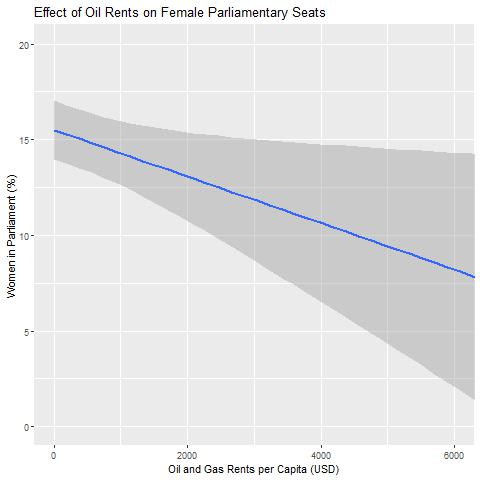
\includegraphics[width=0.8\textwidth]{figure2.jpeg}

\newpage

\subsection*{Figure 3}
\lstinputlisting[language=R, firstline=219, lastline=228]{replication_KC.R}

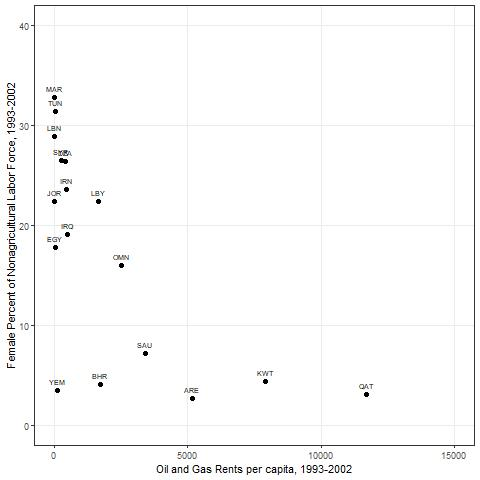
\includegraphics[width=0.8\textwidth]{figure3.jpeg}

\newpage

\subsection*{Figure 4}
\lstinputlisting[language=R, firstline=232, lastline=242]{replication_KC.R}

\begin{center}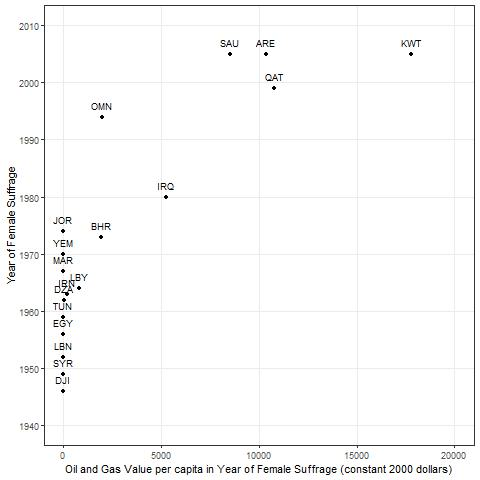
\includegraphics[width=0.75\textwidth]{figure4.jpeg}\end{center}

\subsection*{Figure 5}

\lstinputlisting[language=R, firstline=246, lastline=254]{replication_KC.R}

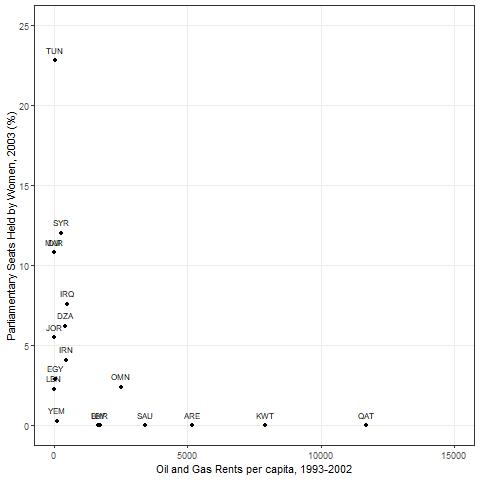
\includegraphics[width=0.8\textwidth]{figure5.jpeg}

\newpage

\subsection*{Figure 6}

\lstinputlisting[language=R, firstline=258, lastline=266]{replication_KC.R}

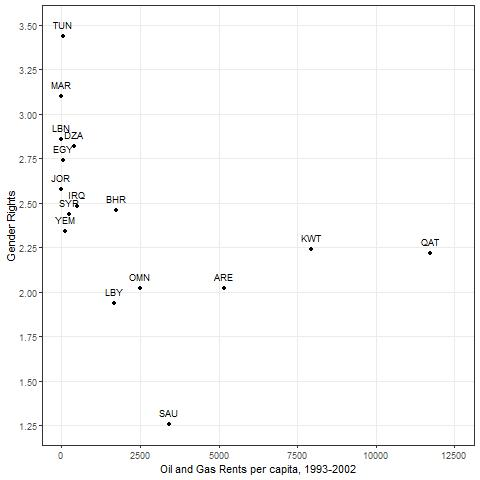
\includegraphics[width=0.8\textwidth]{figure6.jpeg}

\newpage

\subsection*{Original Results: Interpretations}

\noindent The tables show that oil rents per capita are significant in predicting female ministerial positions, parliamentary seats held by women, female nonagricultural labor force participation, and total female labor force participation. The plots visually suggest that (within the Middle East) higher oil and gas rents per capita is associated with lower gender rights, lower percentage of parliamentary seats held by women, and later year of female suffrage. The results support Ross's theory that oil rents are negatively associated with female labor force participation and political participation.

\noindent 

\vspace{.5cm}

\section*{My Contribution}

\vspace{.5cm}

\subsection*{Looking at Natural Resources Rent}

\vspace{.5cm}

\noindent Ross theorizes that oil would negatively impact women's participation in the labor force based on the Dutch Disease Model. This theory is an extension of the resource curse, suggesting that an oil boom encourages an economic shift from trade to non-trade sector, which women are more likely to be excluded from. I questioned if this phenomena would apply to other natural resources, not just oil. To analyze this, I replaced oil rents with natural resource rents in the analysis. 

\vspace{.5cm}

\noindent Data Processing: For the natural resource rent data, if possible, the 2002 data would be used, corresponding with the original study. However, if the 2002 data is unavailable, the 1960-2002 (the years examined in the study) average will be used instead. The natural resource rent data was merged with Ross's data and the z-score was taken, to standardize the data in accordance with Ross's methodology.

\vspace{.5cm}

\lstinputlisting[language=R, firstline=271, lastline=298]{replication_KC.R}

\subsection*{Table 1:}

\lstinputlisting[language=R, firstline=302, lastline=322]{replication_KC.R}

\begin{table*}[!htbp] \centering 
	\label{} 
	\begin{tabular}{@{\extracolsep{5pt}}lcc} 
		\\[-1.8ex]\hline 
		\hline \\[-1.8ex] 
		& \multicolumn{2}{c}{\textit{Dependent variable:}} \\ 
		\cline{2-3} 
		\\[-1.8ex] & \multicolumn{2}{c}{Female Labor Force Participation} \\ 
		\\[-1.8ex] & (1) & (2)\\ 
		\hline \\[-1.8ex] 
		Income (log) & $-$1.864$^{***}$ & $-$1.512$^{**}$ \\ 
		& (0.654) & (0.678) \\ 
		& & \\ 
		Income squared (log) & 2.122$^{***}$ & 1.765$^{***}$ \\ 
		& (0.648) & (0.669) \\ 
		& & \\ 
		Working Age & $-$0.350$^{***}$ & $-$0.428$^{***}$ \\ 
		& (0.119) & (0.126) \\ 
		& & \\ 
		Middle East & $-$0.326$^{***}$ & $-$0.378$^{***}$ \\ 
		& (0.090) & (0.093) \\ 
		& & \\ 
		Communist & 0.286$^{***}$ & 0.307$^{***}$ \\ 
		& (0.082) & (0.086) \\ 
		& & \\ 
		Islam & $-$0.139 & $-$0.164$^{*}$ \\ 
		& (0.086) & (0.089) \\ 
		& & \\ 
		Oil Rents per Capita & $-$0.210$^{***}$ &  \\ 
		& (0.072) &  \\ 
		& & \\ 
		Natural Resource Rents per Capita &  & $-$0.070 \\ 
		&  & (0.074) \\ 
		& & \\ 
		Constant & $-$0.012 & $-$0.013 \\ 
		& (0.060) & (0.062) \\ 
		& & \\ 
		\hline \\[-1.8ex] 
		Observations & 167 & 163 \\ 
		R$^{2}$ & 0.427 & 0.402 \\ 
		Adjusted R$^{2}$ & 0.401 & 0.375 \\ 
		Residual Std. Error & 0.776 (df = 159) & 0.796 (df = 155) \\ 
		F Statistic & 16.898$^{***}$ (df = 7; 159) & 14.912$^{***}$ (df = 7; 155) \\ 
		\hline 
		\hline \\[-1.8ex] 
		\textit{Note:}  & \multicolumn{2}{r}{$^{*}$p$<$0.1; $^{**}$p$<$0.05; $^{***}$p$<$0.01} \\ 
	\end{tabular} 
\end{table*} 

\newpage
\subsection*{Table 2:}
\lstinputlisting[language=R, firstline=325, lastline=346]{replication_KC.R}

\begin{table}[!htbp] \centering 
	\label{} 
	\begin{tabular}{@{\extracolsep{5pt}}lcc} 
		\\[-1.8ex]\hline 
		\hline \\[-1.8ex] 
		& \multicolumn{2}{c}{\textit{Dependent variable:}} \\ 
		\cline{2-3} 
		\\[-1.8ex] & \multicolumn{2}{c}{Parliamentary Seats Held by Women (percent), 2002} \\ 
		\\[-1.8ex] & (1) & (2)\\ 
		\hline \\[-1.8ex] 
		Income (log) & $-$1.748$^{**}$ & $-$1.481$^{*}$ \\ 
		& (0.733) & (0.765) \\ 
		& & \\ 
		Income squared (log) & 2.163$^{***}$ & 1.894$^{**}$ \\ 
		& (0.728) & (0.756) \\ 
		& & \\ 
		Working Age & $-$0.090 & $-$0.218 \\ 
		& (0.134) & (0.144) \\ 
		& & \\ 
		Middle East & $-$0.122 & $-$0.160 \\ 
		& (0.100) & (0.102) \\ 
		& & \\ 
		Communist & 0.140 & 0.194$^{*}$ \\ 
		& (0.095) & (0.100) \\ 
		& & \\ 
		Islam & $-$0.147 & $-$0.167 \\ 
		& (0.100) & (0.104) \\ 
		& & \\ 
		Oil Rents per Capita & $-$0.259$^{***}$ &  \\ 
		& (0.079) &  \\ 
		& & \\ 
		Natural Resource Rents per Capita &  & $-$0.170$^{**}$ \\ 
		&  & (0.085) \\ 
		& & \\ 
		Constant & $-$0.015 & $-$0.011 \\ 
		& (0.068) & (0.071) \\ 
		& & \\ 
		\hline \\[-1.8ex] 
		Observations & 160 & 156 \\ 
		R$^{2}$ & 0.305 & 0.278 \\ 
		Adjusted R$^{2}$ & 0.273 & 0.244 \\ 
		Residual Std. Error & 0.854 (df = 152) & 0.879 (df = 148) \\ 
		F Statistic & 9.513$^{***}$ (df = 7; 152) & 8.128$^{***}$ (df = 7; 148) \\ 
		\hline 
		\hline \\[-1.8ex] 
		\textit{Note:}  & \multicolumn{2}{r}{$^{*}$p$<$0.1; $^{**}$p$<$0.05; $^{***}$p$<$0.01} \\ 
	\end{tabular} 
\end{table} 

\newpage
\subsection*{Table 3:}
\lstinputlisting[language=R, firstline=350, lastline=371]{replication_KC.R}

\begin{table}[!htbp] \centering 
	\caption*{Female Ministers (2002): Oil Model and Natural Resources Model} 
	\label{} 
	\begin{tabular}{@{\extracolsep{5pt}}lcc} 
		\\[-1.8ex]\hline 
		\hline \\[-1.8ex] 
		& \multicolumn{2}{c}{\textit{Dependent variable:}} \\ 
		\cline{2-3} 
		\\[-1.8ex] & \multicolumn{2}{c}{Ministerial Seats Held by Women (percent) 2002} \\ 
		\\[-1.8ex] & (1) & (2)\\ 
		\hline \\[-1.8ex] 
		Income (log) & $-$0.516 & $-$0.446 \\ 
		& (0.810) & (0.825) \\ 
		& & \\ 
		Income squared (log) & 0.894 & 0.817 \\ 
		& (0.803) & (0.815) \\ 
		& & \\ 
		Working Age & $-$0.151 & $-$0.227 \\ 
		& (0.154) & (0.158) \\ 
		& & \\ 
		Middle East & $-$0.171 & $-$0.179 \\ 
		& (0.118) & (0.117) \\ 
		& & \\ 
		Communist & $-$0.110 & $-$0.070 \\ 
		& (0.107) & (0.109) \\ 
		& & \\ 
		Islam & $-$0.029 & $-$0.036 \\ 
		& (0.120) & (0.122) \\ 
		& & \\ 
		Oil Rents per Capita & $-$0.145 &  \\ 
		& (0.088) &  \\ 
		& & \\ 
		Natural Resource Rents per Capita &  & $-$0.145 \\ 
		&  & (0.093) \\ 
		& & \\ 
		Constant & $-$0.010 & $-$0.005 \\ 
		& (0.076) & (0.077) \\ 
		& & \\ 
		\hline \\[-1.8ex] 
		Observations & 154 & 151 \\ 
		R$^{2}$ & 0.174 & 0.165 \\ 
		Adjusted R$^{2}$ & 0.134 & 0.124 \\ 
		Residual Std. Error & 0.933 (df = 146) & 0.939 (df = 143) \\ 
		F Statistic & 4.383$^{***}$ (df = 7; 146) & 4.042$^{***}$ (df = 7; 143) \\ 
		\hline 
		\hline \\[-1.8ex] 
		\textit{Note:}  & \multicolumn{2}{r}{$^{*}$p$<$0.1; $^{**}$p$<$0.05; $^{***}$p$<$0.01} \\ 
	\end{tabular} 
\end{table} 

\newpage

\subsection*{Plots}

\noindent Prepare data
\lstinputlisting[language=R, firstline=376, lastline=382]{replication_KC.R}

\newpage

\subsection*{Plot 1}
\lstinputlisting[language=R, firstline=384, lastline=393]{replication_KC.R}

\begin{center}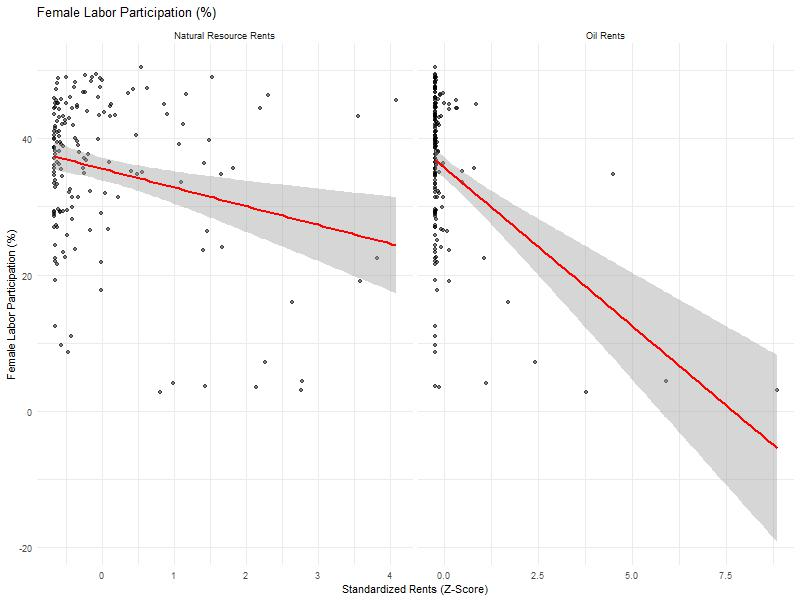
\includegraphics[width=1\textwidth]{Female_Labor.jpeg}\end{center}

\newpage

\subsection*{Plot 2}
\lstinputlisting[language=R, firstline=395, lastline=404]{replication_KC.R}

\begin{center}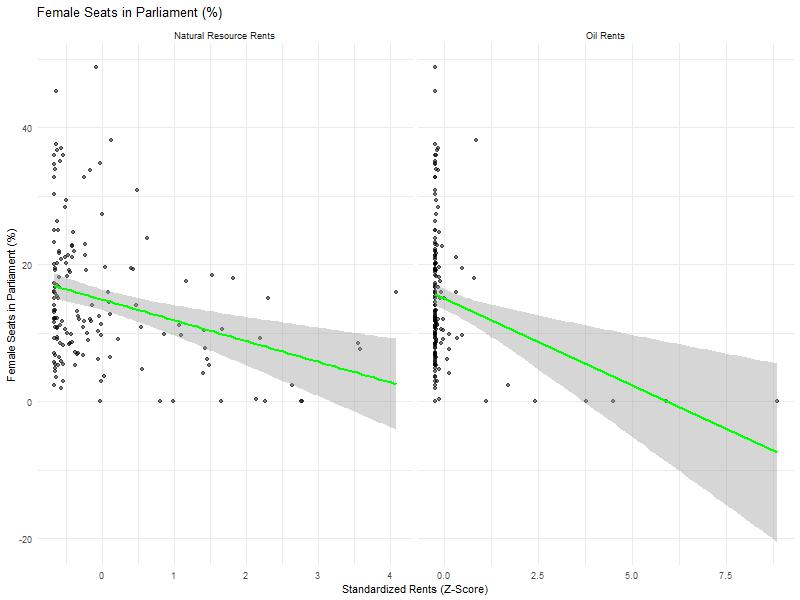
\includegraphics[width=1\textwidth]{Female_Seats.jpeg}\end{center}

\newpage

\subsection*{Plot 3}
\lstinputlisting[language=R, firstline=406, lastline=415]{replication_KC.R}

\begin{center}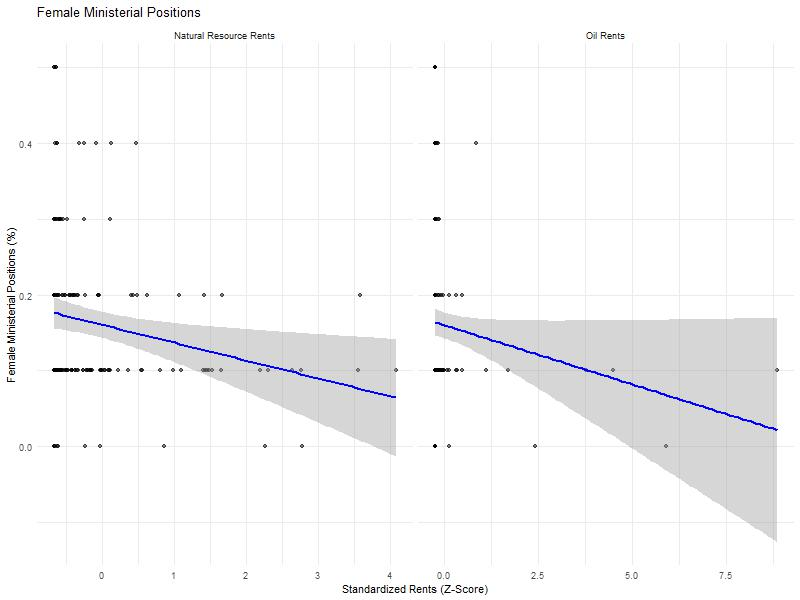
\includegraphics[width=1\textwidth]{Female_Ministers.jpeg}\end{center}

\newpage

\section*{Conclusion}

\vspace{.5cm}

\noindent My results from Table 1 show that Natural Resource Rents per Capita are not significant in predicting Female Labor Force Participation. However, when Natural Resource Rents per Capita are included, Islam becomes significant at a 10 percent significance threshold (it was not significant in the oil rent model). The second table shows that both Oil Rents per Capita and Natural Resource Rents per Capita are significant in predicting the percentage of parliamentary seats held by women. However, Oil Rents per Capita are more significant. Additionally, in the model with Natural Resource Rents per Capita, Communist became significant at a 10 percent significance threshold. Finally, in Table 3, neither Oil Rents per Capita nor Natural Resource Rents per Capita are significant in predicting Ministerial Seats Held by Women.

\vspace{.5cm}

\noindent The plot of Female Labor Participation shows that Oil Rents has a significantly steeper negative slope than Natural Resource Rents. However, Oil Rents has an only slightly steeper slope when plotting the percent of Female Seats in Parliament and an identical slope when plotting percent of Female Ministerial Positions. 

\vspace{.5cm}

\noindent While Natural Resource Rents, was not as significant as Oil Rents in predicting political and labor gender inequality, that result is informative. These results correspond with the assumption that Ross is making that the resource curse is not equal. Some natural resources (like oil) have a greater impact on female labor and political inclusion than others. However, further research is needed to examine the mechanisms behind this relationship and whether these results would hold in further studies. In particular, it would be informative to see if the relationship would be upheld if the study were updated with current data.

\end{document}
